\chapter{Casi di studio e risultati}
\label{ch:casi_studio_e_risultati}

Nei capitoli precedenti la pipeline è stata testata su un primo modello utilizzato come caso di studio per descriverne le singole fasi. 

Adesso vediamo come si comporta la pipeline su altri modelli e quali altri problemi possono esistere.

% =======================================
% Secondo caso di studio
% =======================================
\section{Secondo caso di studio}
\label{sec:caso_studio_2}

Il secondo modello considerato è mostrato in Figura~\ref{fig:cad_caso_2_originale}.
\begin{figure}[htbp]
	\centering
	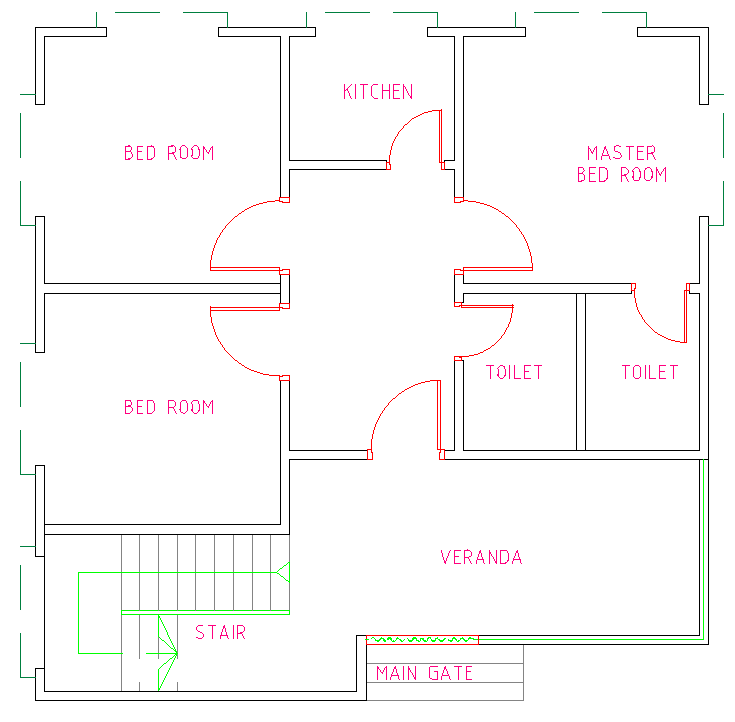
\includegraphics[width=0.5\textwidth]{figures/5_risultati/caso_studio_2/cad_1.png}
	\caption{Modello CAD del secondo caso di studio prima del preprocessing.}
	\label{fig:cad_caso_2_originale}
\end{figure}

Il preprocessing consiste nel rinominare i layer e i blocchi secondo la convenzione imposta e nel rimuovere quelli non utili. Il risultato è mostrato in Figura~\ref{fig:cad_caso_2_preprocessing}.
\begin{figure}[htbp]
	\centering
	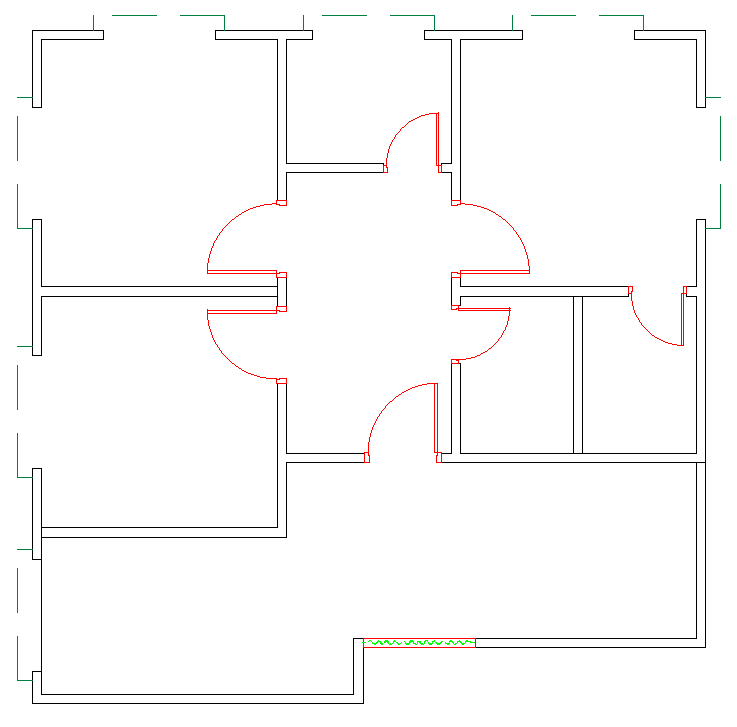
\includegraphics[width=0.5\textwidth]{figures/5_risultati/caso_studio_2/cad_2.png}
	\caption{Modello CAD dopo la rinomina di layer e blocchi e la rimozione degli elementi non utili. In verde, il rumore presente all'interno del rettangolo della porta d'ingresso.}
	\label{fig:cad_caso_2_preprocessing}
\end{figure}

Rimane infine da eliminare il rumore (in verde) presente all'interno del rettangolo della porta d'ingresso.

La pipeline viene eseguita con i seguenti parametri:
\begin{itemize}
	\item \texttt{unit scale} $= 0.1$
	\item \texttt{snap eps} $= 0.01$ (tolleranza $\epsilon$ per il collasso dei vertici, Sezione \ref{sec:collasso_dei_vertici});
	\item \texttt{cluster num samples} $= 30$ e \texttt{cluster eps} $= 0.5$ (parametri di DBSCAN per il riconoscimento delle finestre, Sezione \ref{sec:ricostruzione_varchi}).
\end{itemize}

Come si osserva in Figura~\ref{fig:plot_faces_caso_2_iniziale}, il risultato non è ancora corretto: una faccia di muro non viene classificata correttamente e, in corrispondenza della porta d'ingresso, sono presenti segmenti che si intrecciano.
\begin{figure}[htbp]
	\centering
	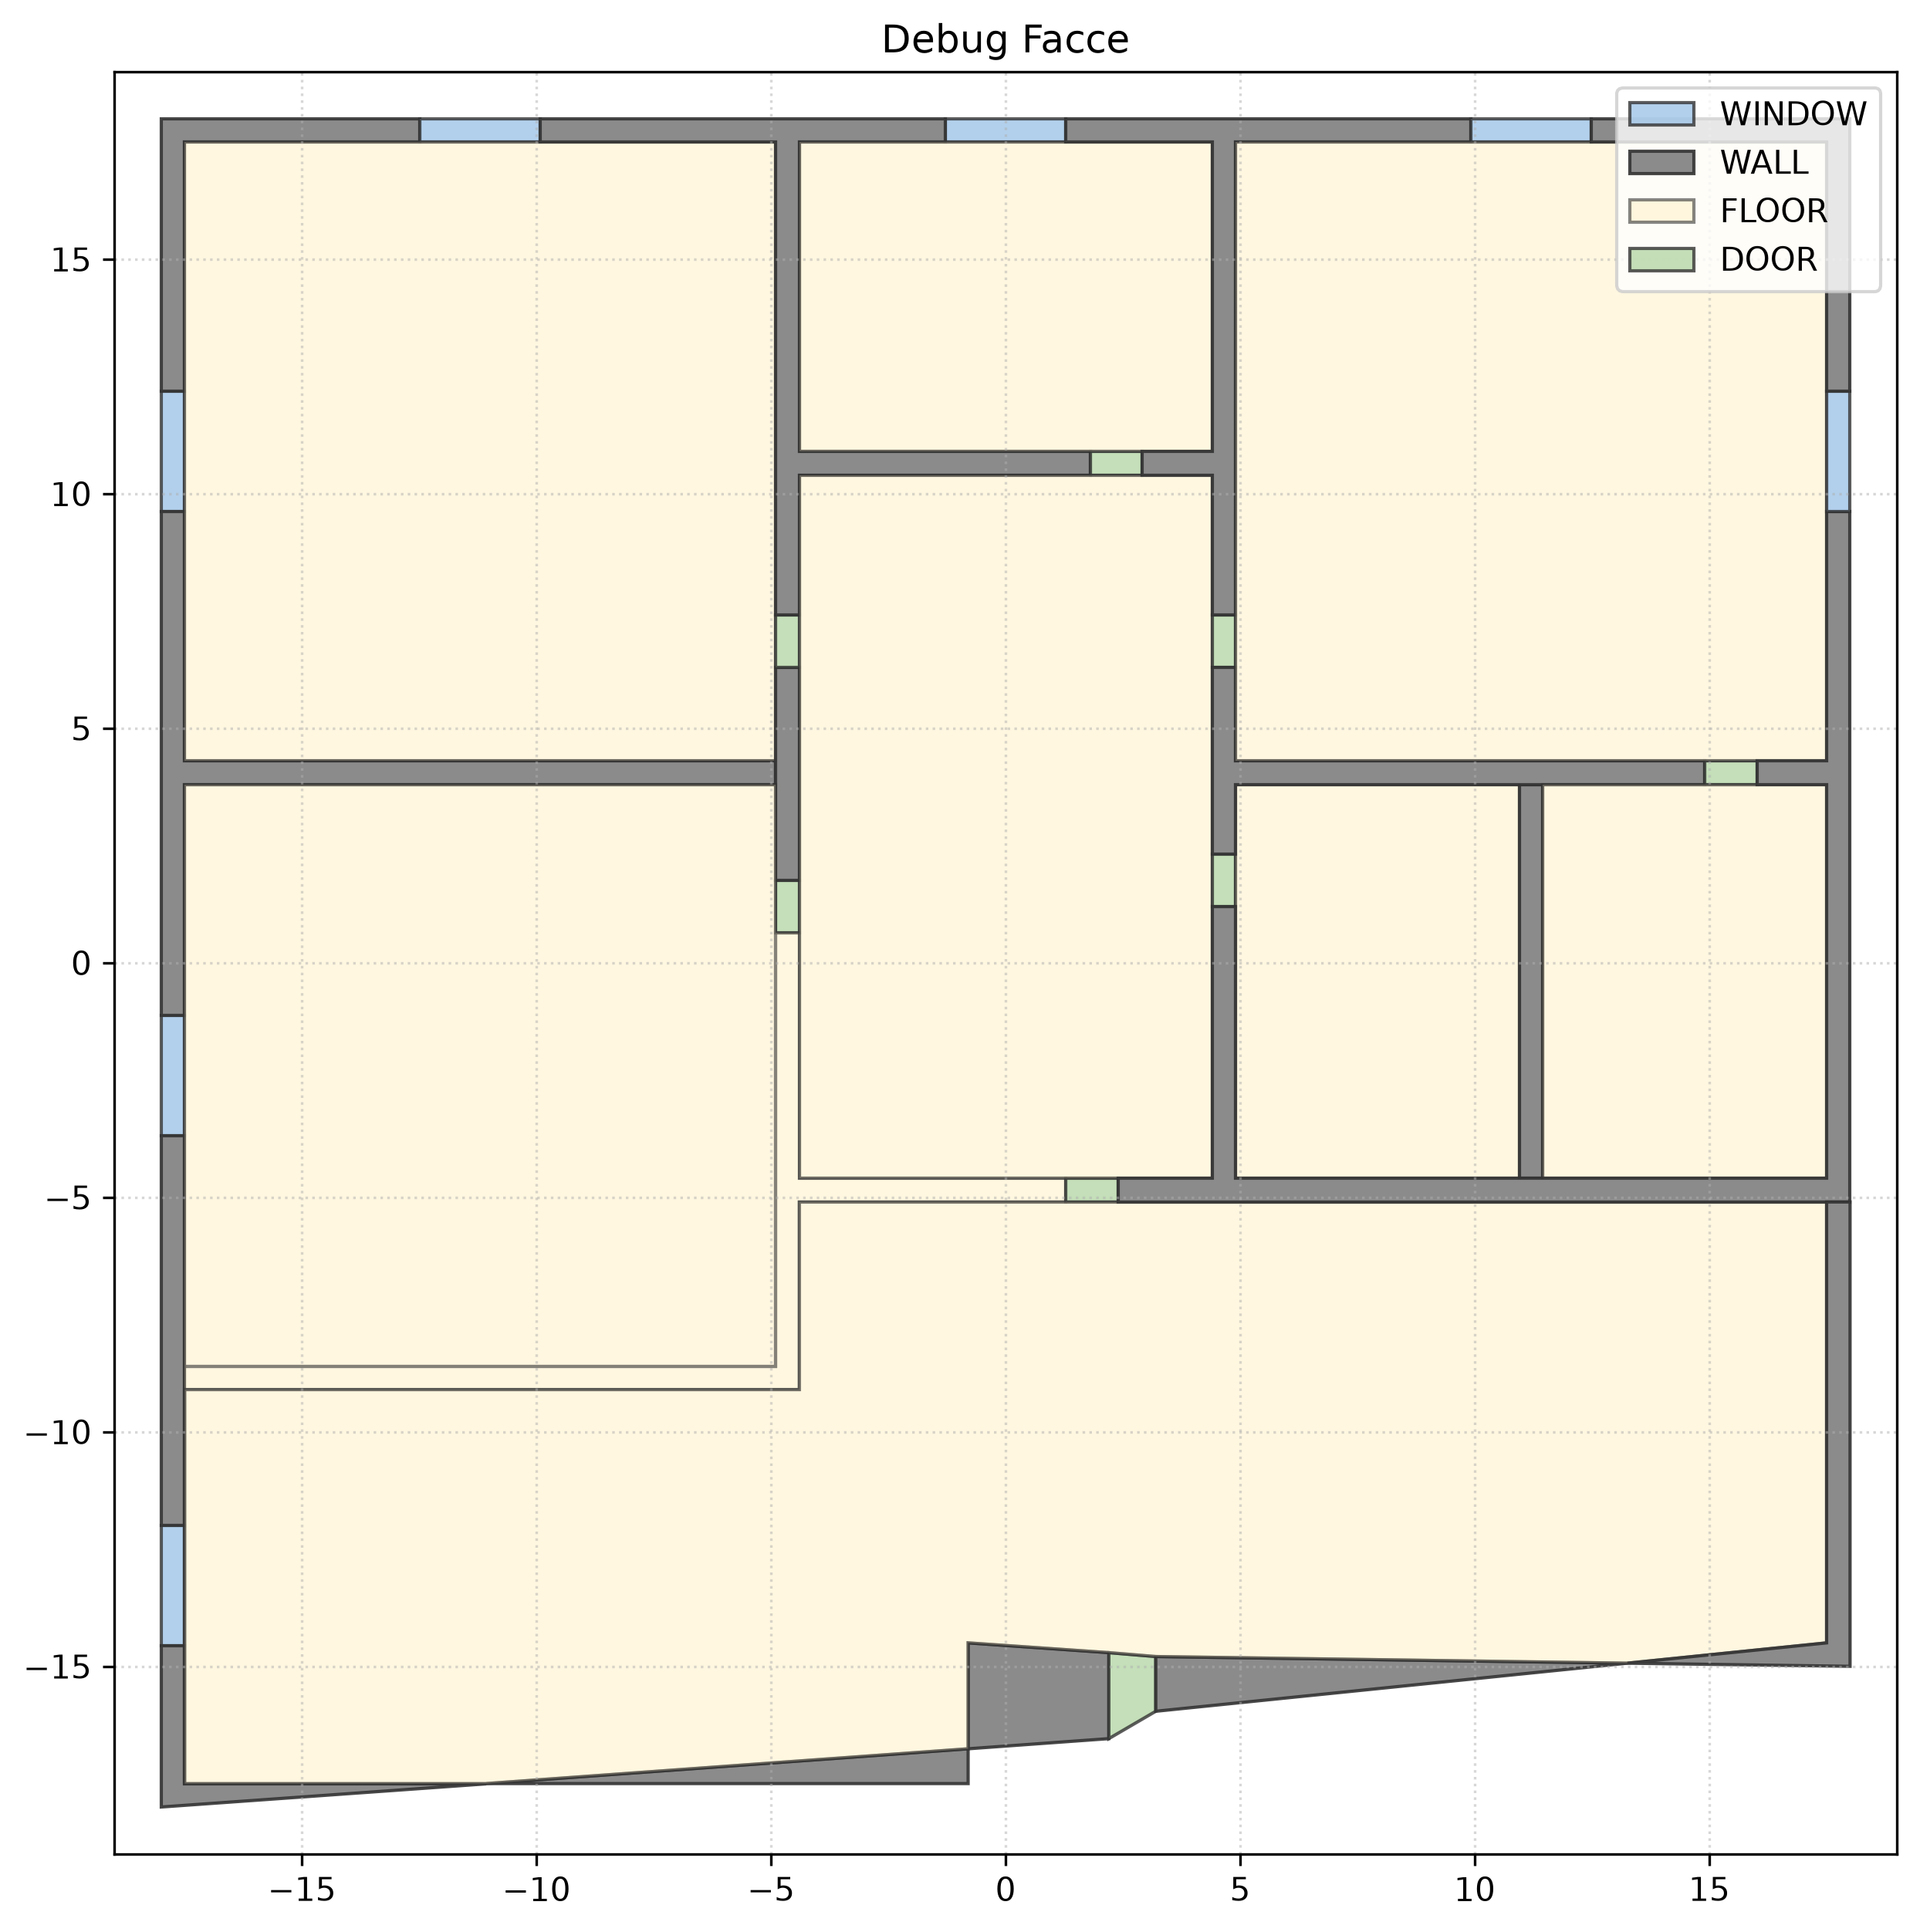
\includegraphics[width=0.5\textwidth]{figures/5_risultati/caso_studio_2/plot_faces.png}
	\caption{Facce estratte al primo tentativo: una faccia di muro non è classificata correttamente e sono presenti segmenti intrecciati in corrispondenza della porta d'ingresso.}
	\label{fig:plot_faces_caso_2_iniziale}
\end{figure}

Il plot delle facce consente di individuare le due cause, entrambe risolvibili intervenendo sul modello CAD in LibreCAD.

\paragraph{Prima correzione.} Nella porzione di muro relativa alla faccia non classificata sono stati rimossi due segmenti e ne sono stati aggiunti due nuovi, così da chiudere correttamente il contorno (Figura~\ref{fig:correzione_1}).
\begin{figure}[htbp]
	\centering
	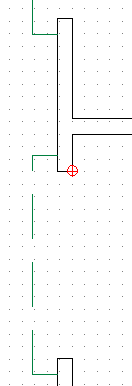
\includegraphics[width=0.15\textwidth]{figures/5_risultati/caso_studio_2/correzione_1.png}
	\caption{Prima correzione: sostituzione di due segmenti sulla porzione di muro non classificata.}
	\label{fig:correzione_1}
\end{figure}

\paragraph{Seconda correzione.} La rappresentazione della porta d'ingresso non è conforme alle assunzioni progettuali (Sezione \ref{sec:assunzioni_progettuali}): le due facce che delimitano il varco non risultano allineate al muro, ma sono rivolte una verso l'alto e l'altra verso sinistra.
Dopo la correzione, la porta assume la forma mostrata in Figura~\ref{fig:correzione_2}.
\begin{figure}[htbp]
	\centering
	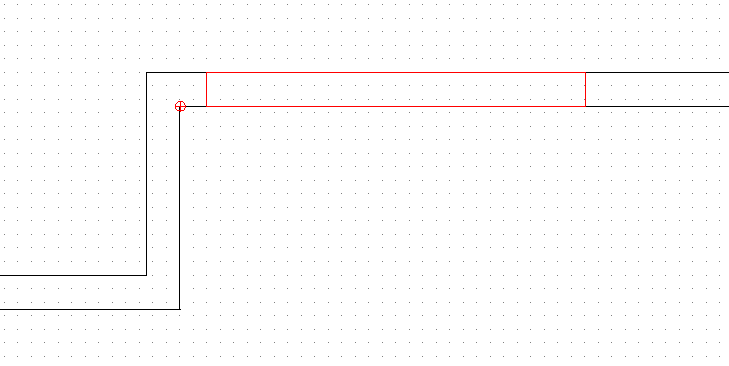
\includegraphics[width=0.40\textwidth]{figures/5_risultati/caso_studio_2/correzione_2.png}
	\caption{Seconda correzione: ridisegno della porta d'ingresso in modo conforme alle assunzioni progettuali.}
	\label{fig:correzione_2}
\end{figure}

Dopo le due correzioni la rappresentazione risulta completa e corretta (Figura~\ref{fig:plot_faces_caso_2_finale}); la Tabella~\ref{tab:statistiche_caso_2} riporta le statistiche dell'esecuzione.
\begin{figure}[htbp]
	\centering
	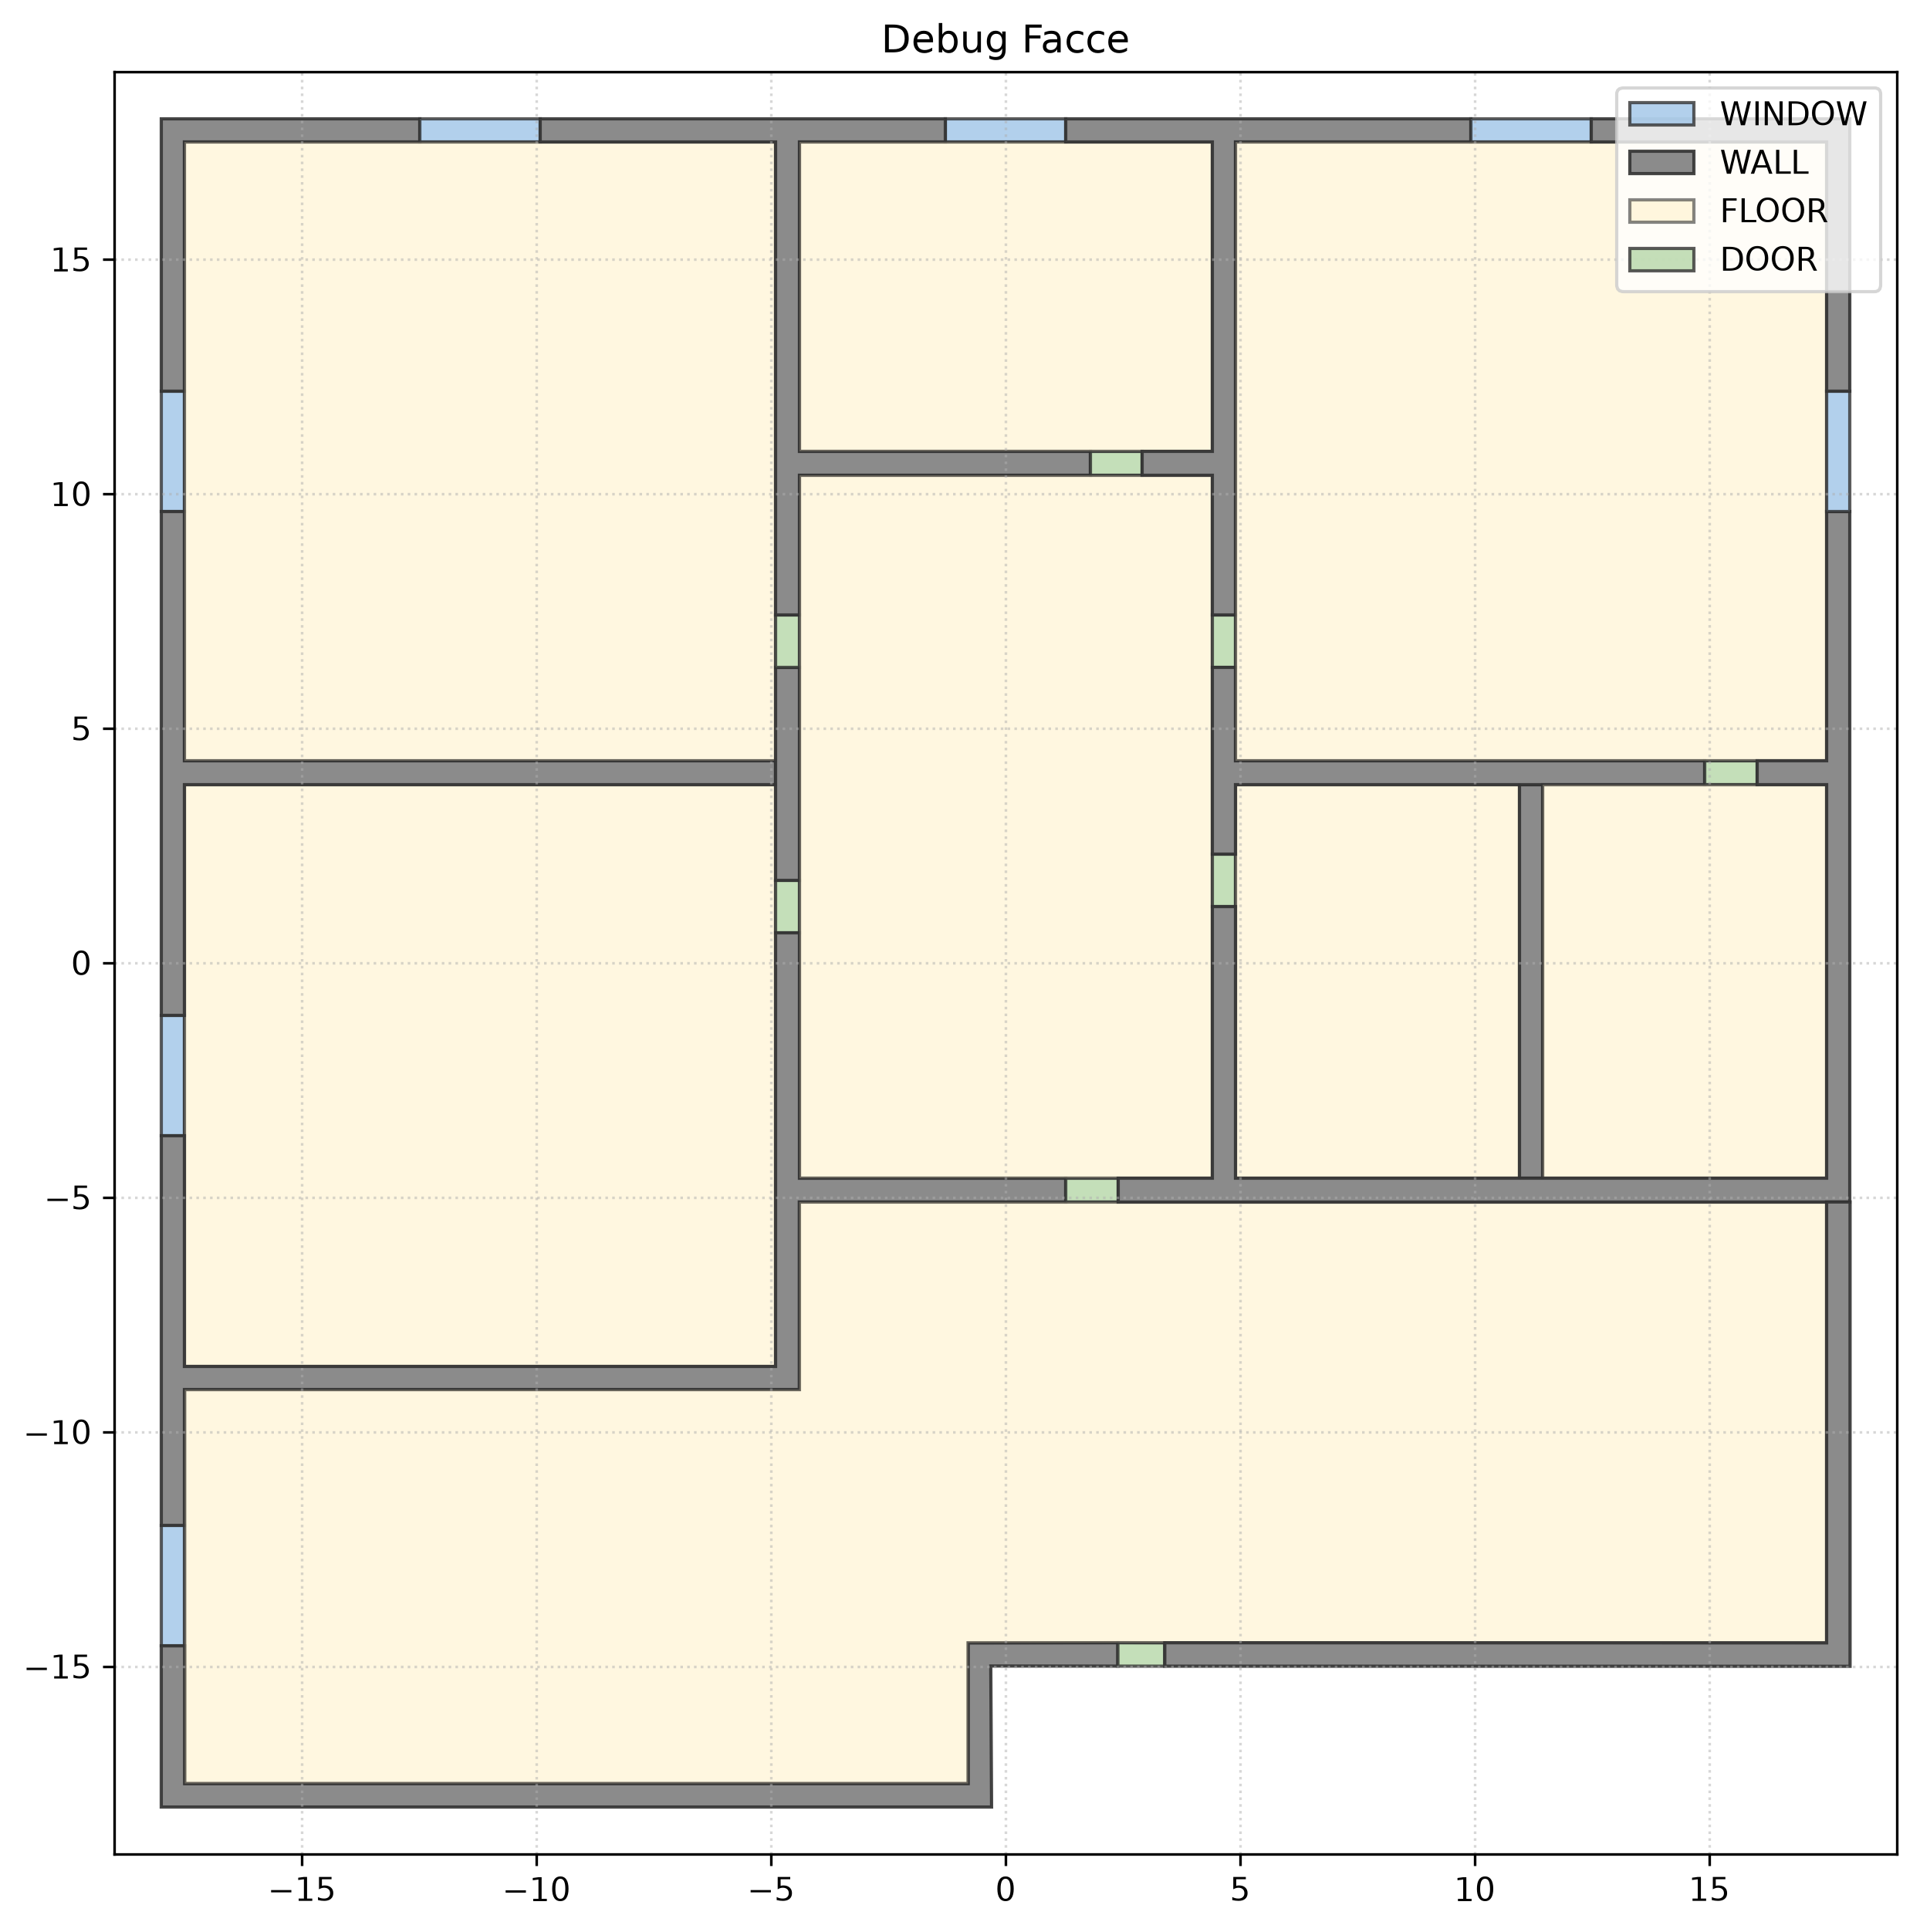
\includegraphics[width=0.5\textwidth]{figures/5_risultati/caso_studio_2/plot_faces_2.png}
	\caption{Facce estratte dopo le correzioni: la classificazione è corretta.}
	\label{fig:plot_faces_caso_2_finale}
\end{figure}

A partire da queste facce è possibile ricostruire il modello ed effettuare il rendering (Figura~\ref{fig:rendering_caso_2}).
\begin{figure}[htbp]
	\centering
	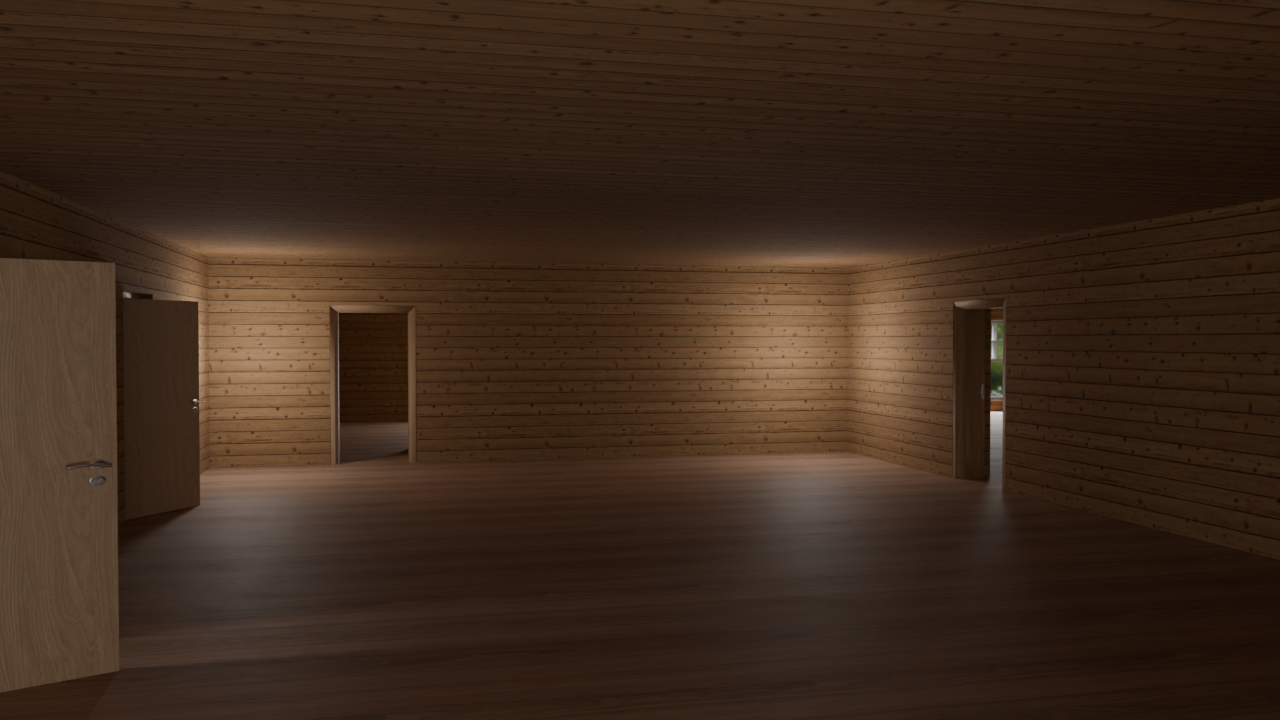
\includegraphics[width=1\textwidth]{figures/5_risultati/caso_studio_2/rendering-1280x720-128-1.png}
	\caption{Rendering (1) del secondo caso di studio ($1280 \times 720$, 128 campioni per pixel).}
	\label{fig:rendering_caso_2}
\end{figure}
\begin{figure}[htbp]
	\centering
	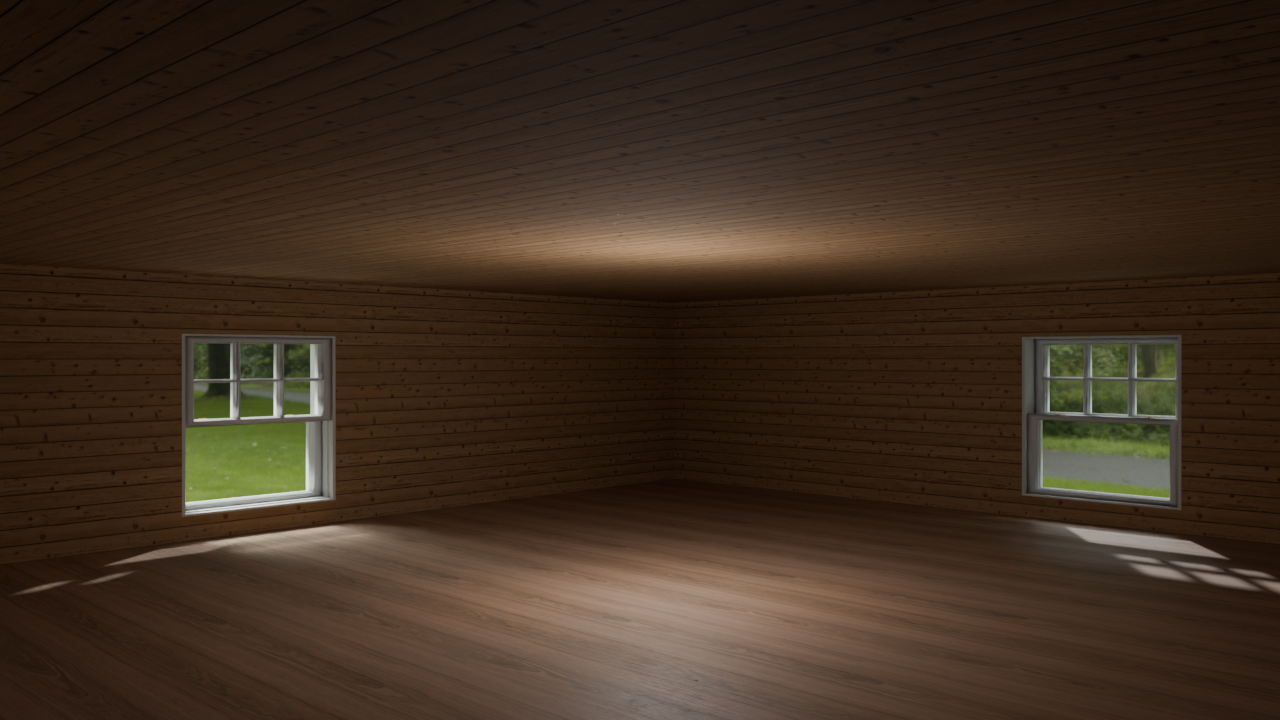
\includegraphics[width=1\textwidth]{figures/5_risultati/caso_studio_2/rendering-1280x720-128-2.png}
	\caption{Rendering (2) del secondo caso di studio}
	\label{fig:rendering2_caso_2}
\end{figure}
\begin{figure}[htbp]
	\centering
	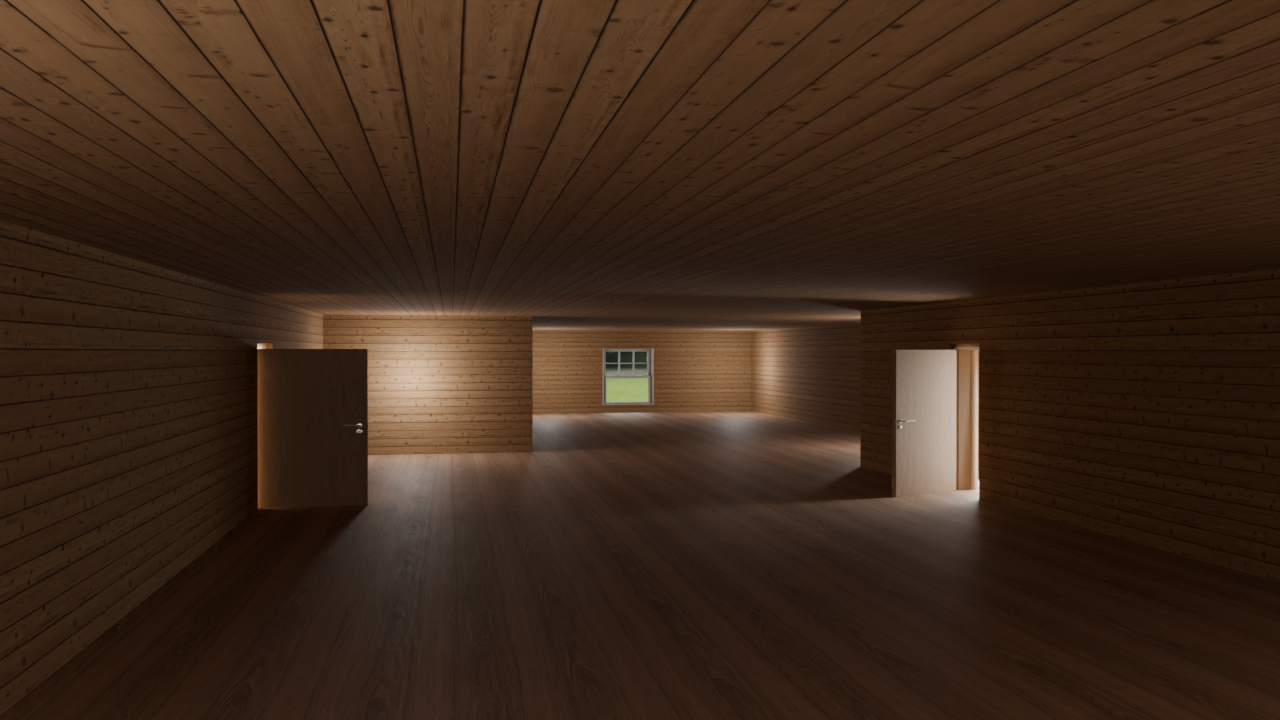
\includegraphics[width=1\textwidth]{figures/5_risultati/caso_studio_2/rendering-1280x720-128-3.png}
	\caption{Rendering (3) del secondo caso di studio}
	\label{fig:rendering3_caso_2}
\end{figure}

Il secondo caso di studio evidenzia che l'osservazione dei plot intermedi, in particolare quello delle facce, è fondamentale per individuare gli errori e capire se intervenire sul modello CAD o sui parametri. In questo caso è stato sufficiente un intervento minimo, la sostituzione di due segmenti e il ridisegno della porta d'ingresso, senza alcuna modifica al codice. 

Ciò conferma però quanto discusso nella Sezione \ref{sec:assunzioni_progettuali}: la qualità del risultato dipende dalla conformità del modello di input alle assunzioni progettuali, e quando queste non sono soddisfatte la correzione resta un'operazione manuale.

\begin{table}[htbp]
	\centering
	\caption{Statistiche dell'esecuzione della pipeline sul secondo caso di studio.}
	\label{tab:statistiche_caso_2}
	\begin{tabular}{lr}
		\hline
		Segmenti duplicati rimossi (muri / porte) & 2 / 1 \\
		Segmenti totali (muro / porta / finestra) & 102 / 8 / 21 \\
		Vertici 2D totali (tutti i segmenti) & 262 \\
		Vertici sui muri prima dello snapping & 204 \\
		Vertici sui muri dopo lo snapping & 105 \\
		Vertici collassati & 99 \\
		Vertici univoci nel grafo finale (2D) & 105 \\
		Punti campionati per il clustering & 651 \\
		Cluster individuati (finestre) & 7 \\
		Facce di muro & 12 \\
		Facce di porta & 8 \\
		Facce di finestra & 7 \\
		Vertici mesh (3D) & 948 \\
		Indici mesh & 1350 \\
		Tempo di esecuzione della pipeline & 5,9 s \\
		\hline
	\end{tabular}
\end{table}

\newpage

% =======================================
% Terzo caso di studio
% =======================================
\section{Terzo caso di studio}
\label{sec:caso_studio_3}

Il terzo modello considerato è \texttt{pincad\_4BHKDuplexHousePlan.dxf} (Figura~\ref{fig:cad_caso_3_originale}).
\begin{figure}[htbp]
	\centering
	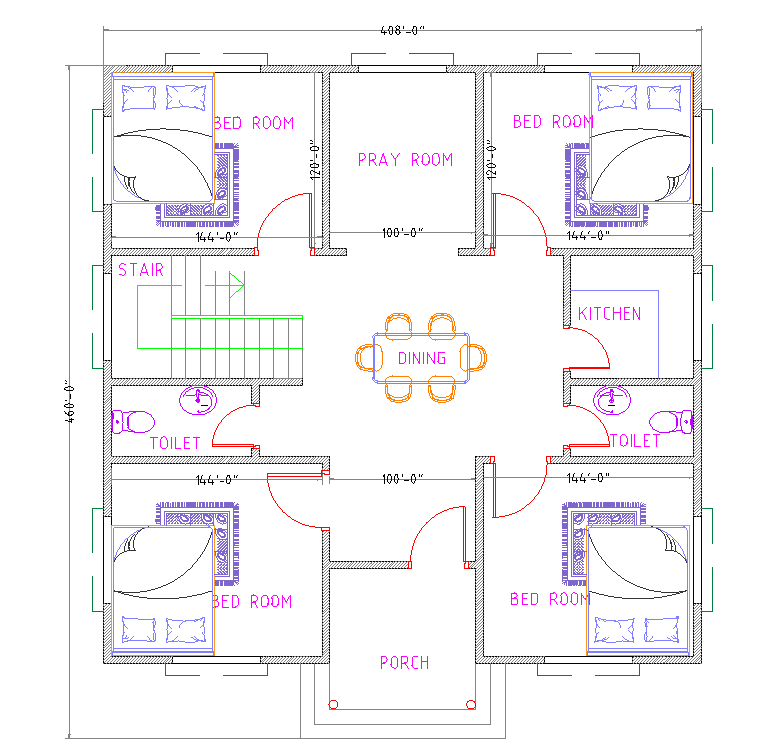
\includegraphics[width=0.5\textwidth]{figures/5_risultati/caso_studio_3/pincad_4BHKDuplexHousePlan.png}
	\caption{Modello CAD del terzo caso di studio.}
	\label{fig:cad_caso_3_originale}
\end{figure}

In questo caso l'unica modifica necessaria consiste nella creazione dei varchi per le finestre: aprendo il modello in LibreCAD si osserva infatti come i muri risultino continui, senza alcuna apertura in corrispondenza delle finestre, in violazione dell'assunzione progettuale secondo cui porte e finestre devono essere rappresentate come aperture nei muri (Sezione \ref{sec:assunzioni_progettuali}). Il modello, una volta corretto, si presenta come mostrato in Figura~\ref{fig:cad_caso_3_corretto}.
\begin{figure}[htbp]
	\centering
	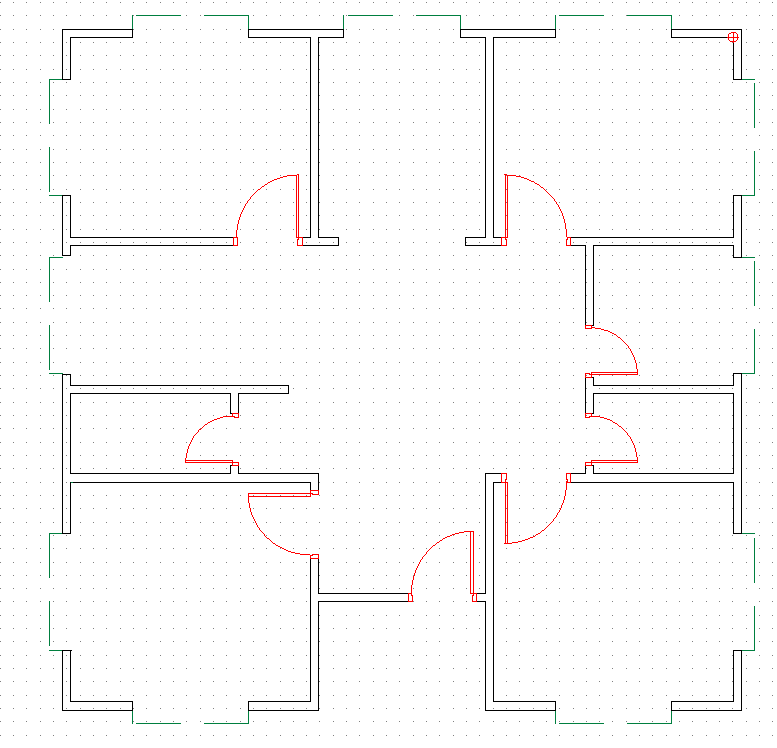
\includegraphics[width=0.5\textwidth]{figures/5_risultati/caso_studio_3/pincad_4BHKDuplexHousePlan_2.png}
	\caption{Modello CAD dopo la creazione manuale dei varchi per le finestre.}
	\label{fig:cad_caso_3_corretto}
\end{figure}

Con questa unica correzione, tutte le facce vengono classificate correttamente (Figura~\ref{fig:plot_faces_caso_3}).
\begin{figure}[htbp]
	\centering
	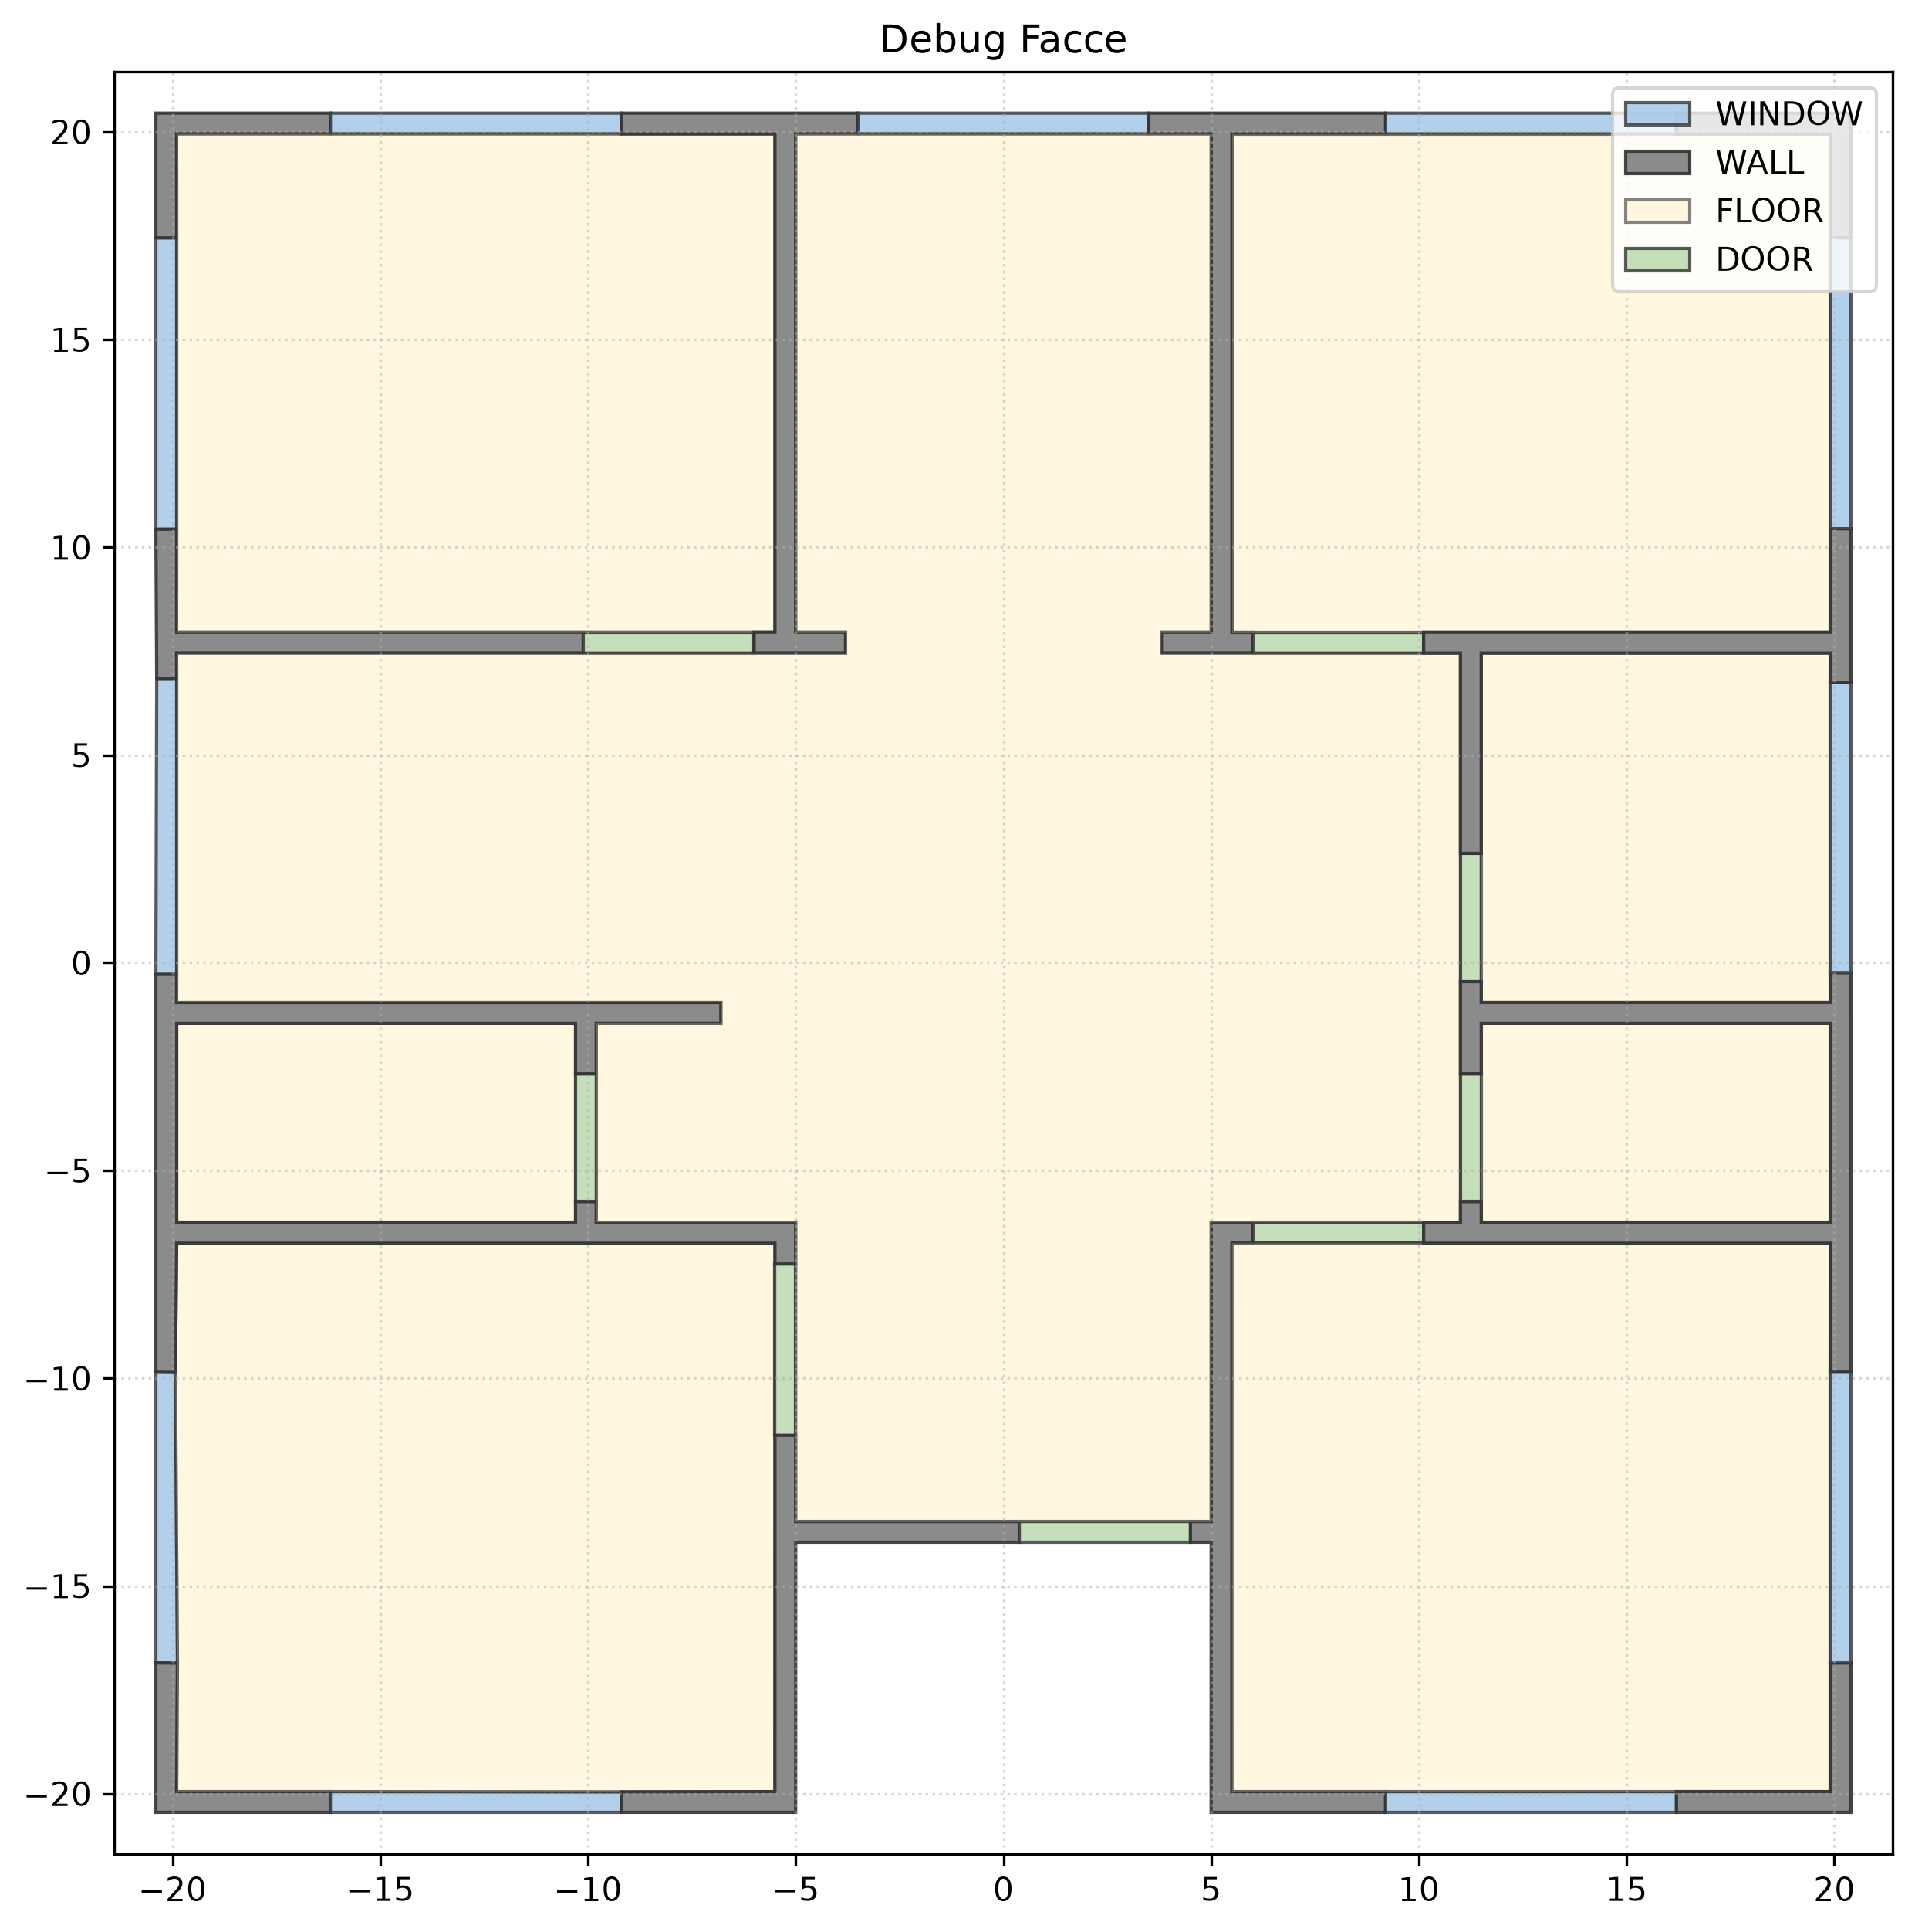
\includegraphics[width=0.5\textwidth]{figures/5_risultati/caso_studio_3/faces.png}
	\caption{Facce estratte e classificate correttamente dopo la correzione.}
	\label{fig:plot_faces_caso_3}
\end{figure}

Il rendering della scena, ottenuto con gli stessi parametri utilizzati nei casi precedenti ($1280 \times 720$, 128 campioni per pixel), è mostrato in Figura~\ref{fig:rendering_caso_3}.
\begin{figure}[htbp]
	\centering
	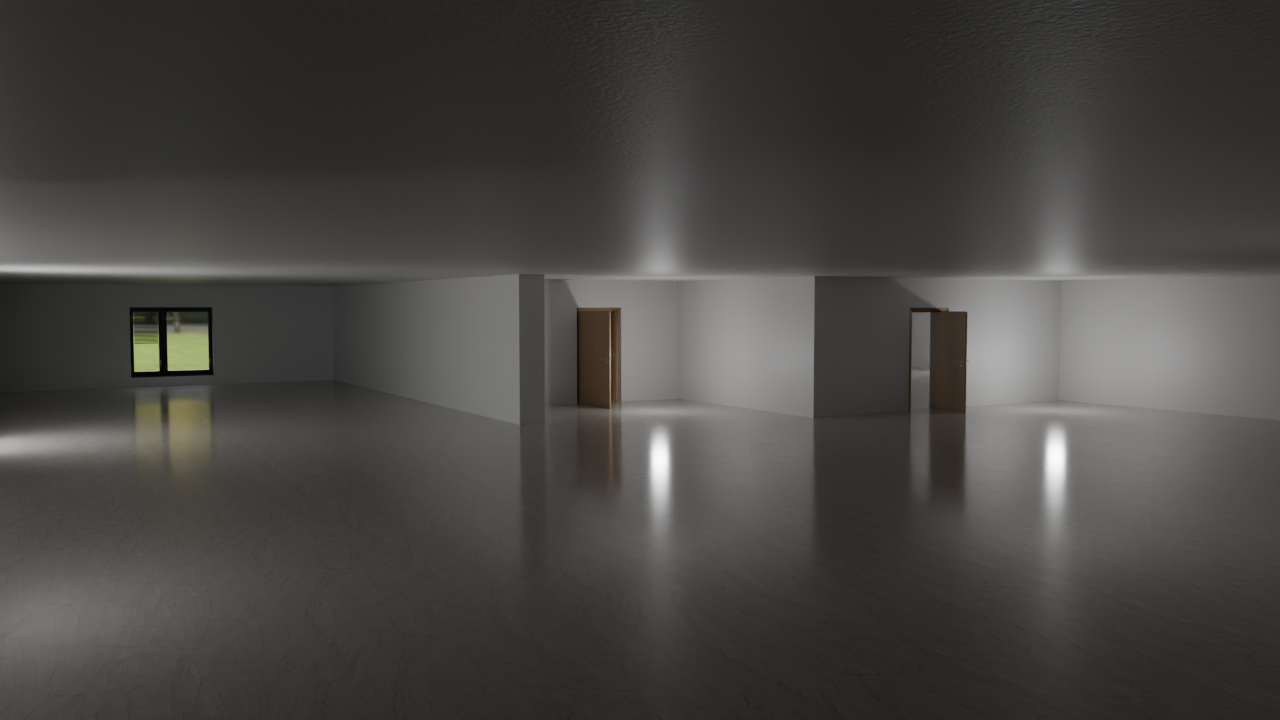
\includegraphics[width=1\textwidth]{figures/5_risultati/caso_studio_3/pincad_4BHKDuplexHousePlan-rendering-1280x720-128-1.png}
	\caption{Rendering (1) del terzo caso di studio ($1280 \times 720$, 128 campioni per pixel).}
	\label{fig:rendering_caso_3}
\end{figure}
\begin{figure}[htbp]
	\centering
	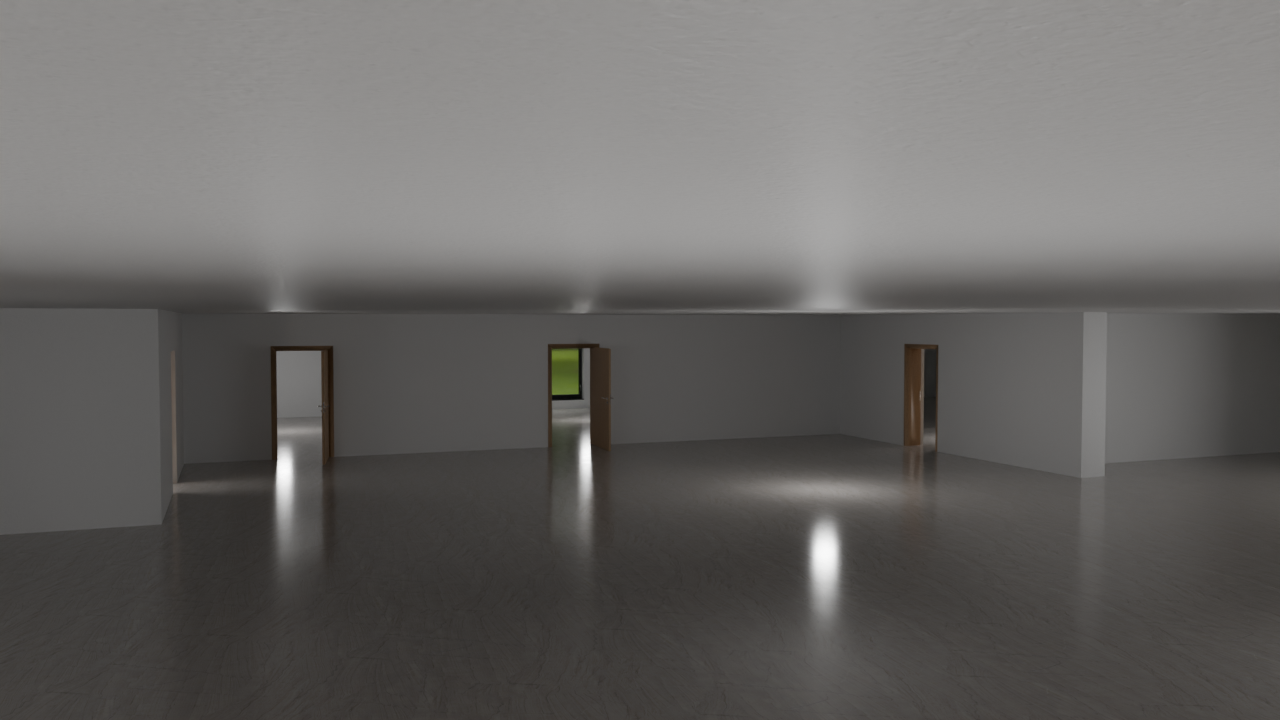
\includegraphics[width=1\textwidth]{figures/5_risultati/caso_studio_3/pincad_4BHKDuplexHousePlan-rendering-1280x720-128-2.png}
	
	\caption{Rendering (2) del terzo caso di studio}
	\label{fig:rendering2_caso_3}
\end{figure}

Rispetto ai casi precedenti, questo modello richiede un intervento manuale minimo e l'introduzione di elementi (i varchi) del tutto assenti nel disegno originale. Ciò conferma come il tipo di intervento richiesto dal preprocessing dipenda fortemente dalla sorgente e dalle convenzioni del singolo modello CAD.

\begin{table}[htbp]
	\centering
	\caption{Statistiche dell'esecuzione della pipeline sul terzo caso di studio.}
	\label{tab:statistiche_caso_3}
	\begin{tabular}{lr}
		\hline
		Segmenti totali (muro / porta / finestra) & 132 / 8 / 33 \\
		Vertici 2D totali (tutti i segmenti) & 346 \\
		Vertici sui muri prima dello snapping & 264 \\
		Vertici sui muri dopo lo snapping & 132 \\
		Vertici collassati & 132 \\
		Vertici univoci nel grafo finale (2D) & 132 \\
		Punti campionati per il clustering & 1023 \\
		Cluster individuati (finestre) & 11 \\
		Facce di muro & 12 \\
		Facce di porta & 8 \\
		Facce di finestra & 11 \\
		Vertici mesh (3D) & 1200 \\
		Indici mesh & 1704 \\
		Tempo di esecuzione della pipeline & 6,0 s \\
		\hline
	\end{tabular}
\end{table}